\documentclass{beamer}
\usepackage{listings}
\usepackage{hyperref,animate}
\usepackage{tikz}
\usetikzlibrary{positioning,shadows,arrows,shapes,calc}
\def\labelenumi\theenumi
\usepackage{graphicx}
\usepackage{amsmath}
\mode<presentation>{\usetheme{Frankfurt}}
\AtBeginSection
{
  \begin{frame}<beamer>
    \frametitle{Outline}
    \tableofcontents[currentsection,currentsubsection]
  \end{frame}
}
\title{Recurrent Neural Nets}
\author{ECE 417: Multimedia Signal Processing\\
Mark Hasegawa-Johnson}
\institute{University of Illinois}
\titlegraphic{\includegraphics{../../../17fall/lectures/imark_1867_bold.png}}
\begin{document}

% Title
\begin{frame}
  \maketitle
\end{frame}

% Title
\begin{frame}
  \tableofcontents
\end{frame}

%%%%%%%%%%%%%%%%%%%%%%%%%%%%%%%%%%%%%%%%%%%%%%%%%%%%%%%%%
\section[FIR/IIR]{Linear Time Invariant Filtering: FIR \& IIR}
\setcounter{subsection}{1}

\begin{frame}
  \frametitle{Basics of DSP: Filtering}
  \[
  y[n] = \sum_{m=-\infty}^\infty h[m] x[n-m]
  \]
  \[
  Y(z)=H(z)X(z)
  \]
\end{frame}

\begin{frame}
  \frametitle{Finite Impulse Response (FIR)}
  \[
  y[n] = \sum_{m=0}^{N-1}h[m]x[n-m]
  \]
  The coefficients, $h[m]$, are chosen in order to optimally position
  the $N-1$ zeros of the transfer function, $r_k$, defined according to:
  \[
  H(z)=\sum_{m=0}^{N-1}h[m] z^{-m}=h[0]\prod_{k=1}^{N-1}\left(1-r_kz^{-1}\right)
  \]
\end{frame}

\begin{frame}
  \frametitle{Infinite Impulse Response (IIR)}
  \[
  y[n] = \sum_{m=0}^{N-1}b_mx[n-m] + \sum_{m=1}^{M-1}a_m y[n-m]
  \]
  The coefficients, $b_m$ and $a_m$, are chosen in order to optimally
  position the $N-1$ zeros and $M-1$ poles of the transfer function,
  $r_k$ and $p_k$, defined according to:
  \[
  H(z)=\frac{\sum_{m=0}^{N-1}b_m z^{-m}}{1-\sum_{m=1}^{M-1}a_m z^{-m}}
  =b_0\frac{\prod_{k=1}^{N-1}\left(1-r_kz^{-1}\right)}{\prod_{k=1}^{M-1}\left(1-p_kz^{-1}\right)}
  \]
  {\bf STABILITY:} If any of the poles are on or outside the unit
  circle ($|p_k|\ge 1$), then $y[n]\rightarrow\infty$, even with
  finite $x[n]$.
\end{frame}

%%%%%%%%%%%%%%%%%%%%%%%%%%%%%%%%%%%%%%%%%%%%%%%%%%%%%%%%%
\section[CNN/RNN]{Nonlinear Time Invariant Filtering: CNN \& RNN}
\setcounter{subsection}{1}

\begin{frame}
  \frametitle{Convolutional Neural Net = Nonlinear(FIR)}
  \centerline{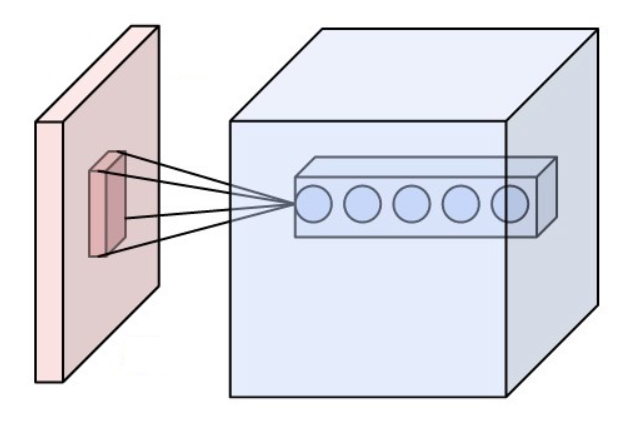
\includegraphics[height=1.5in]{Conv_layer.png}}
  \begin{tiny}Image CC-SA-4.0  by Aphex34, \url{https://commons.wikimedia.org/wiki/File:Conv_layer.png}\end{tiny}
\end{frame}

\begin{frame}
  \frametitle{Convolutional Neural Net = Nonlinear(FIR)}
  \[
  \hat{y}[n] = g\left(\sum_{m=0}^{N-1}w[m]x[n-m]\right)
  \]
  The coefficients, $w[m]$, are chosen to minimize some kind of error.
  For example, suppose that the goal is to make $\hat{y}[n]$ resemble a
  target signal $y[n]$; then we might use 
  \[
  E = \frac{1}{2}\sum_{n=0}^N\left(\hat{y}[n]-y[n]\right)^2
  \]
  and choose
  \[
  w[n] \leftarrow w[n]-\eta\frac{dE}{dw[n]}
  \]
\end{frame}

\begin{frame}
  \frametitle{Recurrent Neural Net (RNN) = Nonlinear(IIR)}
  \centerline{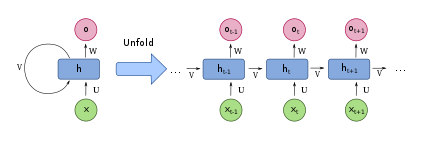
\includegraphics[width=4.5in]{Recurrent.png}}
  \begin{tiny}Image CC-SA-4.0  by Ixnay, \url{https://commons.wikimedia.org/wiki/File:Recurrent_neural_network_unfold.svg}\end{tiny}
\end{frame}

\begin{frame}
  \frametitle{Recurrent Neural Net (RNN) = Nonlinear(IIR)}
  \[
  \hat{y}[n] = g\left(x[n] + \sum_{m=1}^{M-1}w[m] y[n-m]\right)
  \]
  The coefficients, $w[m]$, are chosen to minimize the error.
  For example, suppose that the goal is to make $\hat{y}[n]$ resemble a
  target signal $y[n]$; then we might use 
  \[
  E = \frac{1}{2}\sum_{n=0}^N\left(\hat{y}[n]-y[n]\right)^2
  \]
  and choose
  \[
  w[m] \leftarrow w[m]-\eta\frac{dE}{dw[m]}
  \]
\end{frame}

%%%%%%%%%%%%%%%%%%%%%%%%%%%%%%%%%%%%%%%%%%%%%%%%%%%%%%%%%
\section[Back-Prop]{Back-Propagation Review}
\setcounter{subsection}{1}

\begin{frame}
  \frametitle{Review: Excitation and Activation}
  \begin{itemize}
    \item The {\bf\em activation} of a hidden node is the output of
      the nonlinearity (for this reason, the nonlinearity is sometimes
      called the {\bf activation function}).  For example, in a
      fully-connected network with outputs $\hat{y}_l$, weights $\vec{w}$,
      bias $b$, nonlinearity $g()$, and hidden node activations
      $\vec{h}$, the activation of the $l^{\textrm{th}}$ output node
      is
      \[
      \hat{y}_l = g\left(b_{l}+\sum_{k=1}^p w_{lk} h_k\right)
      \]
    \item The {\bf\em excitation} of a hidden node is the input of the
      nonlinearity.  For example, the excitation of the node above is
      \[
      e_l=b_{l}+\sum_{k=1}^p w_{lk} h_k
      \]
  \end{itemize}
\end{frame}

\begin{frame}
  \frametitle{Backprop = Derivative w.r.t. Excitation}
  \begin{itemize}
    \item The {\bf\em excitation} of a hidden node is the input of the
      nonlinearity.  For example, the excitation of the node above is
      \[
      e_l = b_{l}+\sum_{k=1}^p w_{lk} h_k
      \]
    \item The gradient of the error w.r.t. the weight is
      \[
      \frac{dE}{d w_{lk}} = \epsilon_lh_k
      \]
      where $\epsilon_l$ is the derivative of the error w.r.t. the
      $l^{\textrm{th}}$ {\bf\em excitation}:
      \[
      \epsilon_l = \frac{dE}{de_l}
      \]
  \end{itemize}
\end{frame}

\begin{frame}
  \frametitle{Backprop for Fully-Connected Network}

  Suppose we have a fully-connected network, with inputs $\vec{x}$,
  weight matrices $W^{(1)}$ and $W^{(2)}$, nonlinearities $g()$ and
  $h()$, and output $\hat{y}$:
  \begin{align*}
    e_k^{(1)} = b_{k}^{(1)}+\sum_j w_{kj}^{(1)} x_j,&~~~~
    h_k = g\left(e_k^{(1)}\right)\\
    e_l^{(2)} = b_{l}^{(2)}+\sum_k w_{lk}^{(2)} h_k,&~~~~
    \hat{y}_l = h\left(e_l^{(2)}\right)
  \end{align*}
  Then the back-prop gradients are the derivatives of $E$ with respect
  to the {\bf\em excitations} at each node:
  \begin{align*}
    \frac{dE}{dw_{lk}^{(2)}} =\epsilon_lh_k,&~~~~\epsilon_l=\frac{dE}{de_l^{(2)}}\\
      \frac{dE}{dw_{kj}^{(1)}}=\delta_kx_j,&~~~~\delta_k=\frac{dE}{de_k^{(1)}}
  \end{align*}
\end{frame}

\begin{frame}
  \frametitle{Back-Prop Example}
  \centerline{\animategraphics[loop,controls,width=4.5in]{10}{exp/h0step}{0}{99}}
\end{frame}

\begin{frame}
  \frametitle{Back-Prop Example}

  Suppose we have the following network:
  \begin{align*}
    h &= \cos(x)\\
    \hat{y} &= \sqrt{1+h^2}
  \end{align*}
  Suppose we need $\frac{d\hat{y}}{dx}$.  We find it as
  \begin{align*}
    \frac{d\hat{y}}{dx} &= \frac{d\hat{y}}{dh}\frac{\partial h}{\partial x}
    = \left(\frac{h}{\sqrt{1+h^2}}\right)\left(-\sin(x)\right)
  \end{align*}    
\end{frame}

\begin{frame}
  \frametitle{Back-Prop Example}
  \centerline{\animategraphics[loop,controls,width=4.5in]{10}{exp/h1step}{0}{99}}
\end{frame}

\begin{frame}
  \frametitle{Back-Prop Example}

  Suppose we have the following network:
  \begin{align*}
    h_0 &= \cos(x)\\
    h_1 &= \frac{1}{\sqrt{2}}\left(h_0^3+\sin(x)\right)\\
    \hat{y} &= \sqrt{h_0^2+h_1^2}
  \end{align*}
  What  is $\frac{d\hat{y}}{dx}$?  How can we compute that?
\end{frame}

\begin{frame}
  \frametitle{Causal Graphs for Neural Networks}

  \centerline{
    \tikzstyle{pre}=[<-,shorten <=1pt,>=stealth',semithick,draw=blue]
    \begin{tikzpicture}[hoop/.style={circle,thick,draw=blue,text=black,
          fill=orange!35!white,text centered,text width=0.25cm}]
      \node[hoop] (x) at (0,0) {$x$};
      \node[hoop] (h0) at (-2,1) {$h_0$} edge[pre] (x);
      \node[hoop] (h1) at (2,2) {$h_1$} edge[pre] (x) edge[pre](h0);
      \draw[dashed] (-2.5,0.5) -- (2.5,0.5);
      \node[hoop] (yhat) at (0,3) {$\hat{y}$} edge[pre](h0) edge[pre](h1);
  \end{tikzpicture}}

  We often show the causal graph for the chain rule using bubbles and
  arrows, as shown above.  You can imagine the chain rule as taking a
  summation along any cut through the causal graph---for example, the
  dashed line shown above.  You take the total derivative from
  $\hat{y}$ to the cut, and then the partial derivative from there
  back to $x$.
  \begin{displaymath}
    \frac{d\hat{y}}{dx} = \sum_{i=0}^{N-1}\frac{d\hat{y}}{dh_i}\frac{\partial h_i}{\partial x}
  \end{displaymath}
\end{frame}

\begin{frame}
  \frametitle{Causal Graphs for Neural Networks}

  \centerline{
    \tikzstyle{pre}=[<-,shorten <=1pt,>=stealth',semithick,draw=blue]
    \begin{tikzpicture}[hoop/.style={circle,thick,draw=blue,text=black,
          fill=orange!35!white,text centered,text width=0.25cm}]
      \node[hoop] (x) at (0,0) {$x$};
      \node[hoop] (h0) at (-2,1) {$h_0$} edge[pre] (x);
      \node[hoop] (h1) at (2,2) {$h_1$} edge[pre] (x) edge[pre](h0);
      \draw[dashed] (-2.5,0.5) -- (2.5,0.5);
      \node[hoop] (yhat) at (0,3) {$\hat{y}$} edge[pre](h0) edge[pre](h1);
  \end{tikzpicture}}
  \begin{displaymath}
    \frac{d\hat{y}}{dx} = \sum_{i=0}^{N-1}\frac{d\hat{y}}{dh_i}\frac{\partial h_i}{\partial x}
  \end{displaymath}
  For each $h_i$, we find the {\bf total derivative} of $\hat{y}$
  w.r.t. $h_i$, multiplied by the {\bf partial derivative} of $h_i$ w.r.t. $x$.
\end{frame}

\begin{frame}
  \frametitle{Back-Prop Example}

  First, we find $\frac{d\hat{y}}{dh_1}$:
  \begin{align*}
    \hat{y} &= \sqrt{h_0^2+h_1^2}
  \end{align*}
  \begin{align*}
    \frac{d\hat{y}}{dh_1} &= \frac{h_1}{\sqrt{h_0^2+h_1^2}}
  \end{align*}
\end{frame}

\begin{frame}
  \frametitle{Back-Prop Example}

  \centerline{
    \tikzstyle{pre}=[<-,shorten <=1pt,>=stealth',semithick,draw=blue]
    \begin{tikzpicture}[hoop/.style={circle,thick,draw=blue,text=black,
          fill=orange!35!white,text centered,text width=0.25cm}]
      \node[hoop] (x) at (0,0) {$x$};
      \node[hoop] (h0) at (-2,1) {$h_0$} edge[pre] (x);
      \node[hoop] (h1) at (2,2) {$h_1$} edge[pre] (x) edge[pre](h0);
      \draw[dashed] (-2.5,1.5) -- (1.5,1.5);
      \node[hoop] (yhat) at (0,3) {$\hat{y}$} edge[pre](h0) edge[pre](h1);
  \end{tikzpicture}}
  Second, back-prop to find $\frac{d\hat{y}}{dh_0}$:
  \begin{align*}
    \frac{d\hat{y}}{dh_0} &=\frac{\partial\hat{y}}{\partial h_0}
    + \frac{d\hat{y}}{d h_1}\frac{\partial h_1}{\partial h_0}
    = \frac{1}{\sqrt{h_0^2+h_1^2}}\left(h_0+\left(\frac{3}{\sqrt{2}}\right)h_0^2h_1\right)
  \end{align*}
\end{frame}

\begin{frame}
  \frametitle{Back-Prop Example}

  \centerline{
    \tikzstyle{pre}=[<-,shorten <=1pt,>=stealth',semithick,draw=blue]
    \begin{tikzpicture}[hoop/.style={circle,thick,draw=blue,text=black,
          fill=orange!35!white,text centered,text width=0.25cm}]
      \node[hoop] (x) at (0,0) {$x$};
      \node[hoop] (h0) at (-2,1) {$h_0$} edge[pre] (x);
      \node[hoop] (h1) at (2,2) {$h_1$} edge[pre] (x) edge[pre](h0);
      \draw[dashed] (-2.5,0.5) -- (2.5,0.5);
      \node[hoop] (yhat) at (0,3) {$\hat{y}$} edge[pre](h0) edge[pre](h1);
  \end{tikzpicture}}
  Third, back-prop to find $\frac{d\hat{y}}{dx}$:
  \begin{align*}
    \frac{d\hat{y}}{dx} &=\frac{d\hat{y}}{dh_1}\frac{\partial h_1}{\partial x}
    + \frac{d\hat{y}}{d h_0}\frac{\partial h_0}{\partial x}\\
    &= \left(\frac{h_1}{\sqrt{h_0^2+h_1^2}}\right)\cos(x)
    - \left(\frac{\left(h_0+\left(\frac{3}{\sqrt{2}}\right)h_0^2h_1\right)}{\sqrt{h_0^2+h_1^2}}\right)
    \sin(x)
  \end{align*}
\end{frame}


%%%%%%%%%%%%%%%%%%%%%%%%%%%%%%%%%%%%%%%%%%%%%%%%%%%%%%%%%
\section[Back-Prop]{Back-Propagation Training for CNN and RNN}
\setcounter{subsection}{1}

\begin{frame}
  \frametitle{Back-Prop in a CNN}
  Suppose we have a convolutional neural net, defined by
  \begin{align*}
    e[n] &= \sum_{m=0}^{N-1}w[m]x[n-m]\\
    \hat{y}[n] &= g\left(e[n]\right)
  \end{align*}
  then 
  \[
  \frac{dE}{dw[m]}=\sum_n \delta[n] x[n-m]
  \]
  where $\delta[n]$ is the back-prop gradient, defined by
  \[
  \delta[n] = \frac{dE}{de[n]}
  \]
\end{frame}

\begin{frame}
  \frametitle{Back-Prop in an RNN}
  Suppose we have a recurrent neural net, defined by
  \begin{align*}
    e[n] &= x[n] + \sum_{m=1}^{M-1}w[m] \hat{y}[n-m]\\
    \hat{y}[n] &= g\left(e[n]\right)
  \end{align*}
  then
  \[
  \frac{dE}{dw[m]} = \sum_n \delta[n] \hat{y}[n-m]
  \]
  where $\hat{y}[n-m]$ is calculated by forward-propagation, and then
  $\delta[n]$ is calculated by back-propagation as
  \[
  \delta[n] = \frac{dE}{de[n]}
  \]
\end{frame}

%%%%%%%%%%%%%%%%%%%%%%%%%%%%%%%%%%%%%%%%%%%%%%%%%%%%%%%%%
\section[BPTT]{Back-Prop Through Time}
\setcounter{subsection}{1}

\begin{frame}
  \frametitle{Partial vs. Full Derivatives}

  For example, suppose we want $\hat{y}[n]$ to be as close as possible to
  some target signal $y[n]$:
  \[
  E = \frac{1}{2}\sum_n \left(\hat{y}[n]-y[n]\right)^2
  \]
  Notice that $E$ depends on $\hat{y}[n]$ in many different ways:
  \[
  \frac{dE}{d\hat{y}[n]}=\frac{\partial E}{\partial \hat{y}[n]}+
  \frac{dE}{d\hat{y}[n+1]}\frac{\partial \hat{y}[n+1]}{\partial \hat{y}[n]}+
  \frac{dE}{d\hat{y}[n+2]}\frac{\partial \hat{y}[n+2]}{\partial \hat{y}[n]}+\ldots
  \]
\end{frame}
\begin{frame}
  \frametitle{Partial vs. Full Derivatives}
  In general,
  \[
  \frac{dE}{d\hat{y}[n]}=\frac{\partial E}{\partial \hat{y}[n]}+
  \sum_{m=1}^\infty\frac{dE}{d\hat{y}[n+m]}\frac{\partial \hat{y}[n+m]}{\partial \hat{y}[n]}
  \]
  where
  \begin{itemize}
    \item $\frac{dE}{d\hat{y}[n]}$ is the total derivative, and includes all
      of the different ways in which $E$ depends on $\hat{y}[n]$.
    \item $\frac{\partial \hat{y}[n+m]}{\partial \hat{y}[n]}$ is the partial
      derivative, i.e., the change in $\hat{y}[n+m]$ per unit change in
      $\hat{y}[n]$ if all of the other variables (all other values of
      $\hat{y}[n+k]$) are held constant.
  \end{itemize}
\end{frame}

\begin{frame}
  \frametitle{Partial vs. Full Derivatives}

  So for example, if
  \[
  E = \frac{1}{2}\sum_n \left(\hat{y}[n]-y[n]\right)^2
  \]
  then the partial derivative of $E$ w.r.t. $\hat{y}[n]$ is 
  \[
  \frac{\partial E}{\partial\hat{y}[n]}= \hat{y}[n]-y[n]
  \]
  and the total derivative of $E$ w.r.t. $\hat{y}[n]$ is 
  \[
  \frac{dE}{d\hat{y}[n]}=\left(\hat{y}[n]-y[n]\right)+
  \sum_{m=1}^\infty\frac{dE}{d\hat{y}[n+m]}\frac{\partial\hat{y}[n+m]}{\partial\hat{y}[n]}
  \]
\end{frame}

\begin{frame}
  \frametitle{Partial vs. Full Derivatives}

  So for example, if
  \[
  \hat{y}[n] =g(e[n]),~~~~e[n]=x[n]+\sum_{m=1}^{M-1}w[m]\hat{y}[n-m]
  \]
  then the partial derivative of $\hat{y}[n+k]$ w.r.t. $\hat{y}[n]$ is 
  \[
  \frac{\partial\hat{y}[n+k]}{\partial\hat{y}[n]}= \dot{g}(e[n+k]) w[k] 
  \]
  where we use the notation $\dot{g}(e)=\frac{dg}{de}$.
\end{frame}

\begin{frame}
  \frametitle{Synchronous Backprop vs. BPTT}

  The basic idea of back-prop-through-time is divide-and-conquer.
  \begin{enumerate}
    \item {\bf Synchronous Backprop:} First, calculate the {\bf\em
      partial derivative} of $E$ w.r.t. the excitation $e[n]$ at time
      $n$, assuming that all other time steps are held constant.
      \[
      \epsilon[n] = \frac{\partial E}{\partial e[n]}
      \]
    \item {\bf Back-prop through time:} Second, iterate backward
      through time to calculate the {\bf\em total derivative}
      \[
      \delta[n] = \frac{dE}{d e[n]}
      \]
  \end{enumerate}
\end{frame}

\begin{frame}
  \frametitle{Synchronous Backprop in an RNN}
  Suppose we have a recurrent neural net, defined by
  \begin{align*}
    e[n] &= x[n] + \sum_{m=1}^{M-1}w[m] \hat{y}[n-m]\\
    \hat{y}[n] &= g\left(e[n]\right)\\
    E &= \frac{1}{2}\sum_n\left(\hat{y}[n]-y[n]\right)^2
  \end{align*}
  then
  \[
  \epsilon[n]=\frac{\partial E}{\partial e[n]} = \left(\hat{y}[n]-y[n]\right) \dot{g}(e[n])
  \]
\end{frame}
  
\begin{frame}
  \frametitle{Back-Prop Through Time (BPTT)}
  Suppose we have a recurrent neural net, defined by
  \begin{align*}
    e[n] &= x[n] + \sum_{m=1}^{M-1}w[m] \hat{y}[n-m]\\
    \hat{y}[n] &= g\left(e[n]\right)\\
    E &= \frac{1}{2}\sum_n\left(\hat{y}[n]-y[n]\right)^2
  \end{align*}
  then
  \begin{align*}
    \delta[n]&=\frac{dE}{de[n]}\\
    &=\frac{\partial E}{\partial e[n]}+
    \sum_{m=1}^{\infty}\frac{dE}{de[n+m]}\frac{\partial e[n+m]}{\partial e[n]}\\
    &=\epsilon[n]+\sum_{m=1}^{M-1}\delta[n+m]\dot{g}(e[n+m])w[m]
  \end{align*}
\end{frame}
  
%%%%%%%%%%%%%%%%%%%%%%%%%%%%%%%%%%%%%%%%%%%%%%%%%%%%%%%%%%%%%%%%%%%%%%%%%%%%%%%%%
\section{Conclusion}
\setcounter{subsection}{1}

\begin{frame}
  \begin{itemize}
  \item Back-Prop, in general, is just the chain rule of calculus:
    \begin{displaymath}
      \frac{dE}{dw} = \sum_{i=0}^{N-1}\frac{dE}{dh_i}\frac{\partial h_i}{\partial w}
    \end{displaymath}
  \item TDNN is a one-dimensional ConvNet, the nonlinear version of an FIR filter.
    Coefficients are shared across time steps.
  \item RNN is the nonlinear version of an IIR filter.  
    Coefficients are shared across time steps.
    Error is back-propagated from every output time step to every input time step.
    \begin{displaymath}
      \delta[n]=\frac{dE}{de[n]}=\frac{\partial E}{\partial e[n]}+
      \sum_{m=1}^{M-1}\delta[n+m]\dot{g}(e[n+m])w[m]
    \end{displaymath}
    \[
    \frac{dE}{dw[m]} = \sum_n \delta[n] \hat{y}[n-m]
    \]
  \end{itemize}
\end{frame}


\end{document}

